%Book
%Copyright (C) 2019  Patrick Diehl
%
%This program is free software: you can redistribute it and/or modify
%it under the terms of the GNU General Public License as published by
%the Free Software Foundation, either version 3 of the License, or
%(at your option) any later version.

%This program is distributed in the hope that it will be useful,
%but WITHOUT ANY WARRANTY; without even the implied warranty of
%MERCHANTABILITY or FITNESS FOR A PARTICULAR PURPOSE.  See the
%GNU General Public License for more details.

%You should have received a copy of the GNU General Public License
%along with this program.  If not, see <http://www.gnu.org/licenses/>.

%----------------------------------------------------------------------------------------
\chapter{Linear algebra}
%----------------------------------------------------------------------------------------
For the topic of linear algebra, we refer to~\cite{hefferonlinear,scheick1997linear}. We focus on vector and matrices and some operations on them, as we need them for example in the finite element method. Note that we look from the computer science perspective on matrices and vectors and focus how efficiently use existing libraries in our code. Several highly optimized C++ linear algebra libraries~\cite{wang2013augem,eigenweb,rupp2016viennacl,sanderson2016armadillo} are available. However, the look into the Blaze library since this library has a HPX backend for parallel computations. 


%----------------------------------------------------------------------------------------
\section{Blaze library}
%----------------------------------------------------------------------------------------
Blaze is an open-source, high-performance C++ math library for dense and sparse arithmetic. With its state-of-the-art Smart Expression Template implementation Blaze combines the elegance and ease of use of a domain-specific language with HPC-grade performance, making it one of the most intuitive and fastest C++ math libraries available. More details about the implementation details~\cite{doi:10.1137/110830125,6266939}.

%----------------------------------------------------------------------------------------
\subsection{Vectors}
\index{Blaze!vector}
\index{Blaze!vector}
\label{sec:linalg:vectors}
%----------------------------------------------------------------------------------------
A $n$ dimensional vector space (or linear space) $\mathbf{u}$ is defined as $\mathbf{u}=(u_1,u_2,\ldots,u_{n-1},u_{n-2})\in \mathbb{R}^n$. In Blaze, a three dimensional vector\link{https://bitbucket.org/blaze-lib/blaze/wiki/Vectors} is defined as \cpp{blaze::DynamicVector<int> c (3UL);}\link{https://bitbucket.org/blaze-lib/blaze/wiki/Vector\%20Types\#!dynamicvector}. Note the Blaze is a template based library as the STL and we have to provide the data type of the vector in the parenthesizes \cpp{<int>} and in the second parenthesizes \cpp{(3UL)} the size of the vector. as for the \cpp{std::vector} we can get the size of the vector by the expression \cpp{c.size()} and to access a value, we use \cpp{auto value = c[i];}. Listing~\ref{code:blaze:vector:iterator} shows how to iterate over a Blaze vector using the access operator \cpp{c[i]} and iterators \cpp{it-value}. For more details on iterators we refer to Section~\ref{ref:stl:iterators}. \\

\begin{lstlisting}[language=c++,caption={Iterating over a Blaze vector using a for loop with iterators.\label{code:blaze:vector:iterator}},float,floatplacement=tb]
#include <blaze/Math.h>

int main()
{
blaze::StaticVector<int,3UL> c{ 4, -2, 5 };

// Loop over the vector
for( size_t i=0UL; i< c.size(); ++i )
   std::cout << c[i] << std::endl;
   
// Iterate over a vector
blaze::CompressedVector<int> d{ 0, 2, 0, 0};
for( CompressedVector<int>::Iterator it=d.begin(); 
  it!=d.end(); ++it ) 
    std::cout << it->value() << std::endl;

}
\end{lstlisting}

For the three dimensional vector space, we look into so some common operations which are often needed in simulations, \emph{e.g.}\ in $N$-body simulation (Section~\ref{sec:nbody}) or peridyanmic simulation (Section~\ref{sec:pd}). For a vector $\mathbf{u}=(x,y,z)\in\mathbb{R}^3$ the norm\index{vector!norm} or length of the vector reads as
\begin{align}
\vert\mathbf{u}\vert = \sqrt{x^2+y^2+z^2}
\end{align}
and its direction is given as $\sfrac{\mathbf{u}}{\vert\mathbf{u}\vert}$. The norm of the vector $\vert c \vert$ is computed in Blaze using the expression \cpp{const double norm = norm( b );}\link{https://bitbucket.org/blaze-lib/blaze/wiki/Vector\%20Operations\#!norms}. The inner product\index{vector!inner product} $\bullet$ reads as
\begin{align}
\mathbf{u}_1 \bullet \mathbf{u}_2 = x_1x_2 + y_1y_2 + z_1z_2\text{.}
\end{align}
Figure~\ref{fig:vector:inner} shows the angle $\Theta$ between the two vectors $\mathbf{u}_1$ and $\mathbf{u}_2$ defined using the inner product $\bullet$.  The inner product $\mathbf{u}_1 \bullet \mathbf{u}_2 $ is computed in Blaze using the expression \cpp{int result2 = inner(v1,v2);}\link{https://bitbucket.org/blaze-lib/blaze/wiki/Vector-Vector\%20Multiplication\#!inner-product-scalar-product-dot-product}. The cross product $\times$ is defined by
\begin{align}
\mathbf{u}_1 \times \mathbf{u}_2 = \vert\mathbf{u}_1 \vert \vert\mathbf{u}_2 \vert sin(\theta) \mathbf{n}
\end{align}
and its geometric interpretation is sketches in Figure~\ref{fig:vector:cross}. The cross product of the two vector is the orthogonal vector on the two vectors. In addition, the norm of the cross product $\vert\textcolor{azure}{\mathbf{u}_1}\times\textcolor{amaranth}{\mathbf{u}_2}\vert$ is the are spanned by the two vectors. A more accessible form is
\begin{align}
\left( \begin{matrix}
c_0 \\ c_1 \\ c_2
\end{matrix}\right) = \left( \begin{matrix}
y_2 z_2 - z_1 x_2 \\
z_1 x_2 - x_1 z_2 \\
x_1 y_2 - y_1x_2
\end{matrix}\right) \text{.}
\end{align}
The inner product $\mathbf{u}_1 \times \mathbf{u}_2 $ is computed in Blaze using the expression \cpp{cross(u1,u2);}.

\begin{figure}[tb]
\begin{subfigure}{.5\textwidth}
\center
\begin{tikzpicture}
\draw [->] (0,0) -- (2,2);
\draw [->] (0,0) -- (2,-2);
\draw [azure,thick,domain=-45:45] plot ({cos(\x)}, {sin(\x)});

\node at (3,0) {$\Theta=\arccos(\sfrac{\mathbf{u_1}\bullet\mathbf{u_2}}{\vert\mathbf{u_1}\vert\vert \mathbf{u_2}\vert})$};
\node[above] at (2,2) {$\mathbf{u}_1$};
\node[below] at (2,-2) {$\mathbf{u}_2$};
\end{tikzpicture}
\caption{The angle $\Theta$ between the two vectors $\mathbf{u}_1$ and $\mathbf{u}_2$ defined using the inner product $\bullet$. }
\label{fig:vector:inner}
\end{subfigure}
\begin{subfigure}{.5\textwidth}
\begin{tikzpicture}
\draw[->,azure,thick] (0,0) -- (2,0);
\draw[->] (0,0) -- (0,2);
\draw[->,amaranth,thick] (0,0) -- (1,1);
\draw (1,1) -- (3,1) -- (2,0);
\draw [black,domain=0:45] plot ({cos(\x)}, {sin(\x)});

\node[below,azure] at (1,0) {$\mathbf{u}_1$};
\node[left,amaranth] at (0.75,0.75) {$\mathbf{u}_2$};
\node[above] at (0,2) {$\textcolor{azure}{\mathbf{u}_1}\times\textcolor{amaranth}{\mathbf{u}_2}$};
\node[above] at (3,1) {$\vert\textcolor{azure}{\mathbf{u}_1}\times\textcolor{amaranth}{\mathbf{u}_2}\vert$};
\node at (0.5,0.25) {$\Theta$};
\end{tikzpicture}
\caption{Visualization of the inner product $\vert\textcolor{azure}{\mathbf{u}_1}\times\textcolor{amaranth}{\mathbf{u}_2}\vert$ which is the orthogonal vector on the two others. }
\label{fig:vector:cross}
\end{subfigure}
\caption{Geometric interpretation of the inner product $\bullet$ (\subref{fig:vector:inner}) and the cross product $\times$ (\subref{fig:vector:cross}).}
\end{figure}


%----------------------------------------------------------------------------------------
\subsection{Matrices}
\index{Blaze!matrix}
%----------------------------------------------------------------------------------------
A matrix $\mathbf{A}\in \mathbb{R}^{n,m}$ has $n$ rows and $m$ columns
\begin{align}
\mathbf{A} = \begin{pmatrix}
a_{1,1} & \ldots & a_{1,m} \\
\vdots & \ldots & \vdots \\
a_{n,1} & \ldots & a_{n,m} 
\end{pmatrix}
\end{align} 
and following matrix operations are defined:
\begin{itemize}
\item Scaling:
\begin{align}
 2 \mathbf{A} = \begin{pmatrix}
2a_{1,1} & \ldots & 2a_{1,m} \\
\vdots & \ldots & \vdots \\
2a_{n,1} & \ldots & 2a_{n,m} 
\end{pmatrix} 
\end{align}
\item Addition:
\begin{align}
\mathbf{A} + \mathbf{B}  = \begin{pmatrix}
a_{1,1} + b_{1,1}  & \ldots & a_{1,m} + b_{1,m} \\
\vdots & \ldots & \vdots \\
a_{n,1} + b_{n,1} & \ldots & a_{n,m} + b_{n,m} 
\end{pmatrix}
\end{align}
\item Matrix vector multiplication
\begin{align}
\mathbf{A}  \mathbf{v}  = \begin{pmatrix}
a_{1,1} * b_{1} + & \ldots & + a_{1,m} * b_{n} \\
\vdots & \ldots & \vdots \\
a_{n,1} * b_{1} + & \ldots & + a_{n,m} * b_{n} 
\end{pmatrix}\text{.}
\end{align}
\end{itemize}
let us look what kind of matrices are provided by Blaze and how to use them for calculations. Let us start with Blaze's matrix types\link{https://bitbucket.org/blaze-lib/blaze/wiki/Matrix\%20Types}, see Listing~\ref{code:blaze:matrix:types}. The first type is the \cpp{DynanmicMatrix<T>}\link{https://bitbucket.org/blaze-lib/blaze/wiki/Matrix\%20Types\#!dynamicmatrix} which is a arbitrary sized matrix with dynamically allocated elements of arbitrary type \cpp{T}. Note that Blaze is a template-based library and the template type is provided within the first braces. For more details for C++ templates, we refer to~\ref{sec:generic:programming}. In the second pair of braces, the dimension of the $n$ and $m$ are given. Note that the values are not initialized of this matrix which means that the values can have any value. For large matrices the \cpp{DynanmicMatrix<T>} matrix is the best option, especially if the dimensions are not known at compile time. If the matrix is small and the dimensions are known at compile time, a \cpp{blaze::StaticMatrix}\link{https://bitbucket.org/blaze-lib/blaze/wiki/Matrix\%20Types\#!staticmatrix} matrix should be used. In Line~7 we define the $3\times 4$ matrix, but do not allocate the memory yet and the matrix has zero rows and columns. Only after calling the constructor the memory is allocated. Note that the dimensions of the matrix are provided as template arguments in that case. All matrices are default row-major matrices and to switch to column-major matrices, the template argument \cpp{blaze::columnMajor} is available. The last matrix type is the \cpp{blaze::CompressedMatrix} which is used for sparse matrices\link{https://bitbucket.org/blaze-lib/blaze/wiki/Matrix\%20Types\#!sparse-matrices} with only few non-zero entries.\\

These are the main types of matrices provided by the Blaze library. However, there are some special purpose matrices which are often needed available. One is the identity matrix \cpp{blaze::IdentityMatrix} with has ones on all diagonal entries and is zero everywhere else. To have a matrix with zero valued elements, the \cpp{blaze::ZeroMatrix} is used.
 
\begin{lstlisting}[language=c++,caption={Blaze matrix types.\label{code:blaze:matrix:types}},float,floatplacement=tb]
// Definition of a 3x4 matrix 
// Values are not initialized
blaze::DynamicMatrix<int> A( 3UL, 4UL );

// Definition of a 3x4 matrix
// with 0 rows and columns
blaze::StaticMatrix<int,3UL,4UL> A;

// Definition of column-major matrix
// with 0 rows and columns
blaze::DynamicMatrix<double,blaze::columnMajor> C;

// Definition of a 3x4 integral row-major matrix
blaze::CompressedMatrix<int> A( 3UL, 4UL );

// Definition of a 3x3 identity matrix
blaze::IdentityMatrix<int> A( 3UL );

// Definition of a 3x5 zero matrix
blaze::ZeroMatrix<int> A( 3UL, 5UL );
\end{lstlisting}

For all matrices the size of the matrix \cpp{size( A )}; returns the total amount of elements $(n \times m)$. The number of rows are obtained by \cpp{M2.rows();} and the number of columns are obtained by \cpp{M2.columns();}. All matrix operations\link{https://bitbucket.org/blaze-lib/blaze/wiki/Matrix\%20Operations} are applied as \cpp{abs( A );} which means the absolute value of all matrix elements is computed. Note that the elements of a Blaze matrix are accessed using different kind of parentheses \cpp{A(0,0) = 1;} sets the first element of the matrix to one.\\

One often used task in linear algebra is decomposition\index{decomposition} of matrices. Blaze implements following decomposition methods: Cholesky~\cite{cholesky2005resolution}, QR/RQ, and QL/LQ. Listing~\ref{code:blaze:decomposition} shows how to use LU~\cite{bunch1974triangular} decomposition method. Note that we do not cover this methods in this course, but it is an important feature you should know. For more details we refer for example to~\cite{press1992numerical}.

\begin{lstlisting}[language=c++,caption={Matrix decomposition methods in Blaze\label{code:blaze:decomposition}},float,floatplacement=tb]
blaze::DynamicMatrix<double,blaze::rowMajor> A;
// ... Resizing and initialization

blaze::DynamicMatrix<double,blaze::rowMajor> L, U, P;

// LU decomposition of a row-major matrix
lu( A, L, U, P );  

assert( A == L * U * P );
\end{lstlisting}

Another important feature is the computation of Eigenvalues\index{eigenvalue} and Eigenvectors\index{eingenvector} which is shown in Listing~\ref{code:blaze:eigen}.  Note that we do not cover this methods in this course, but it is an important feature you should know. For more details we refer for example to~\cite{press1992numerical}. 

\begin{lstlisting}[language=c++,caption={Matrix decomposition methods in Blaze\label{code:blaze:eigen}},float,floatplacement=tb]

// The symmetric matrix A
SymmetricMatrix< DynamicMatrix<double,rowMajor>> 
    A( 5UL, 5UL );  
// ... Initialization

// The vector for the real eigenvalues
DynamicVector<double,columnVector> w( 5UL );    
// The matrix for the left eigenvectors   
DynamicMatrix<double,rowMajor>     V( 5UL, 5UL );  

eigen( A, w, V );
\end{lstlisting}







%----------------------------------------------------------------------------------------
\subsubsection{Application}
%----------------------------------------------------------------------------------------
One application of matrices is communication between a group of people $P_1,\ldots,P_4$. Figure~\ref{fig:matrix:application:graph} shows the communication network of these four people as a directed graph. For example $P_1$ communications with $P_2$ and $P_4$. One question one can ask, is how long does it take to transfer a message from $P_3$ to $P_2$. To obtain this information, we can use a adjacency matrix~\cite{biggs1993algebraic} as in Equation~\eqref{eq:graph:matrix} where a matrix element $a_{1,2}=1$ means that there is an edge in the graph from $P_1$ to $P_2$. By doing this for all people in our group, we will get this matrix. This matrix will tell us that $P_1$ has contact with $P_2$ and $P_4$, $P_2$ with $P_3$ and so on.

\begin{align}
\mathbf{M} = \left\lbrace\begin{matrix}
0 & 1 & 0 & 1 \\
0 & 0 & 1 & 0 \\
1 & 0 & 0 & 1 \\
1 & 1 & 0 & 0
\end{matrix} \right\rbrace
\label{eq:graph:matrix}
\end{align}

To compute how knows the message after four cycles, we define
\begin{center}
$\mathbf{M}^4 = \mathbf{M} \cdot \mathbf{M} \cdot \mathbf{M} \cdot \mathbf{M} $,  
\end{center}
which means for $\mathbf{M}^n$, we have to do $n$ multiplications of $\mathbf{M}$. After the multiplications, we get following result
\begin{align*}
M^2 = \left\lbrace\begin{matrix}
1 &  1 & 1 &  0 \\
1 & 0 & 0  & 1 \\
1 & 2 & 0 & 1 \\
0 & 1 & 1 & 1
\end{matrix} \right\rbrace
\end{align*}
and see that person $P_3$ can send some message to Person $P_2$ in two cycles. For more applications, we refer to~\cite{scheick1997linear}. 

\begin{exercise}
Transfer the matrix in Equation~\ref{eq:graph:matrix} into a Blaze matrix and try to reproduce the resulting matrix by multiplying the matrix four times.
\end{exercise}

\begin{figure}[tb]
\centering
\begin{tikzpicture}
  \SetGraphUnit{3}
  \Vertex{P1}
  \WE(P1){P2}
  \WE(P2){P3}
  \WE(P3){P4}
  %
  \Edge(P1)(P2)
  \Edge(P1)(P4)
  \Edge(P2)(P3)
  \Edge(P3)(P1)
  \Edge(P3)(P4)
  \Edge(P4)(P1)
  \Edge(P4)(P2)
\end{tikzpicture}
\caption{Graph of the communication network.}
\label{fig:matrix:application:graph}
\end{figure}

%----------------------------------------------------------------------------------------
\section{Compiling code using Blaze}
%----------------------------------------------------------------------------------------
To use Blaze, we have to first install the library on our system\link{https://bitbucket.org/blaze-lib/blaze/wiki/Configuration\%20and\%20Installation}. Listing~\ref{code:blaze:inst:cmake} shows how to install Blaze using CMake and Listing~\ref{code:blaze:inst:manually} how to install Blaze manually. Note that you should check if there is a newer version of Blaze available.

\begin{minipage}{\linewidth}
\begin{minipage}{0.45\linewidth}
\begin{lstlisting}[language=bash,caption={Installing Blaze using CMake.\label{code:blaze:inst:cmake}}]
tar -xvf blaze-3.6.tar.gz
cd blaze-3.6
cmake -DCMAKE_INSTALL_PREFIX=/home/patrick/blaze .
make install
\end{lstlisting}
\end{minipage}
\hfill
\begin{minipage}{0.45\linewidth}
\begin{lstlisting}[language=bash,,caption={Installing Blaze manually.\label{code:blaze:inst:manually}}]
tar -xvf blaze-3.6.tar.gz
cd blaze-3.6
cp -r ./blaze /home/patrick/blaze
\end{lstlisting}
\end{minipage}
\end{minipage}

After installing Blaze, we can use preferable CMake, see Listing~\ref{code:blaze:compile:cmake}, or compile the code by hand, see Listing~\ref{code:blaze:compile:manually}. For more details about CMake, we refer to Section~\ref{sec:cmake}. Note that we have already installed Blaze on the server and there is no need to install Blaze on your own device.

\begin{minipage}{\linewidth}
\begin{minipage}{0.45\linewidth}
\begin{lstlisting}[language=bash,caption={Compilation using CMake.\label{code:blaze:compile:cmake}}]
find_package( blaze )
if( blaze_FOUND )
   add_library( blaze_target INTERFACE )
   target_link_libraries( blaze_target 
   	INTERFACE blaze::blaze )
endif()
\end{lstlisting}
\end{minipage}
\hfill
\begin{minipage}{0.45\linewidth}
\begin{lstlisting}[language=bash,,caption={Manually compilation.\label{code:blaze:compile:manually}}]
g++ -I/home/diehlpk/blaze BlazeTest.cpp
\end{lstlisting}
\end{minipage}
\end{minipage}

Currently, we only have compiled Blaze for serial execution. To compile Blaze with C++ 11 threads, we have to add following arguments \bash{-std=c++11 -DBLAZE_USE_CPP_THREADS} to the compiler and export following environment variable \bash{export BLAZE_NUM_THREADS=4  // Unix systems}. For HPX parallelism, we have to add following arguments \bash{-DBLAZE_USE_HPX_THREADS} to the compiler and run \bash{./a.out --hpx:threads=4} to use four threads. Fore more details, we refer to~\link{https://bitbucket.org/blaze-lib/blaze/wiki/Shared\%20Memory\%20Parallelization}.

%----------------------------------------------------------------------------------------
\chapter{Solvers}
%----------------------------------------------------------------------------------------
Another important task in applied mathematics is to solve linear equations systems. Before we dig into the numerical and implementation details, we look into one example we know from our school lessons in mathematics. Figure~\ref{fig:example:interesction} plots the two functions $f_1(x_1)=-\sfrac{3}{2}x_1+1$ and  $f_2(x_1)=-\sfrac{2}{6}x_1-\sfrac{8}{6}$. From a visual perspective one can see that the intersection of these two functions is at $(2,-2)$. However, for more complex functions or more degree of freedoms the visual approach can get cumbersome. Another approach is to formulate the corresponding linear equations systems and solve it to get the intersections. For the linear equation system, we want to have the both functions in the form $3x_1+2x_2=2$ and $2X_1+6x_2=-8$ which are just a different way to write $f_1(x_1)$ and $f_2(x_1)$. Now we want to define a matrix $\mathbf{M}$ and the right-hand side $\mathbf{b}$ to find the solution $\mathbf{x}$ as $\mathbf{M}\mathbf{x}=\mathbf{b}$. Using the second form the function representation, we get 
\begin{align}
\mathbf{M}\mathbf{x}&=\mathbf{b} \\
\left(\begin{matrix}
3 & 2 \\
2 & 6 \\
\end{matrix}\right)
\left(\begin{matrix}
x_1 \\
x_2
\end{matrix}\right)
&=\left(
\begin{matrix}
2 \\
-8
\end{matrix}\right)\text{.}
\end{align}
We know from school how to solve the matrix using Gaussian elimination~\cite{brown1999contextual}\index{Gaussian elimination}. In Equation~\eqref{eq:gauss:1} the first line is multiplied by two and the second line by three to get the same factor in the first column. In Equation~\eqref{eq:gauss:2} we can subtract the first line from the second line to get a zero in the second line. In Equation~\eqref{eq:gauss:3} we now can get the value for $x_2$ because we know $2x_2=-28\rightarrow x_2=-2$. In Equation~\eqref{eq:gauss:4} the first line is multiplied by seven and the second line by two to get the same factor in the second column. In Equation~\eqref{eq:gauss:5} the second row is subtracted from the first one. In Equation~\eqref{eq:gauss:6} we now can get the value for $x_1$ because we know $42x_1=84\rightarrow x_2=2$. Which is the same solution as visual obtained in Figure~\ref{fig:example:interesction}.\\

Note that one can implement the Gauss elimination, but the theoretical complexity of this algorithm is $\mathcal{O}(n^3)$ where $n$ is the number of unknowns~\cite{farebrother1988linear}. So this algorithm is feasible for thousands of unknown, but might not scale for millions of unknowns. Fore more details about the complexity, we refer to~\cite{fang1997worst}. In that case the so-called iterative methods are used. We will look into the Conjugate Gradient method in the next section. For more details about iterative methods\index{iterative methods} we refer to~\cite{olshanskii2014iterative,briggs2000multigrid}.


\begin{align}
\left(\begin{matrix}
3 & 2 \\
2 & 6 \\
\end{matrix}\right)
\left(\begin{matrix}
x_1 \\
x_2
\end{matrix}\right)
&=\left(
\begin{matrix}
2 \\
-8
\end{matrix}\right)
\quad \left|\begin{matrix}
\cdot 2 \\
\cdot 3
\end{matrix}\right. \label{eq:gauss:1}\\
\left(\begin{matrix}
6 & 4 \\
6 & 18 \\
\end{matrix}\right)
\left(\begin{matrix}
x_1 \\
x_2
\end{matrix}\right)
&=\left(
\begin{matrix}
4 \\
-24
\end{matrix}\right)
\quad\left|\begin{matrix}
 \\
- R1 \\
\end{matrix}\right. \label{eq:gauss:2} \\
\left(\begin{matrix}
6 & 4 \\
0 & 14 \\
\end{matrix}\right)
\left(\begin{matrix}
x_1 \\
x_2
\end{matrix}\right)
&=\left(
\begin{matrix}
4 \\
-28
\end{matrix}\right) 
\quad \left|\begin{matrix}
 \\
\rightarrow x_2 = -2
\end{matrix}\right. \label{eq:gauss:3} \\
\left(\begin{matrix}
6 & 4 \\
0 & 14 \\
\end{matrix}\right)
\left(\begin{matrix}
x_1 \\
x_2
\end{matrix}\right)
&=\left(
\begin{matrix}
4 \\
-28
\end{matrix}\right) 
\quad \left|\begin{matrix}
\cdot 7 \\
\cdot 2
\end{matrix}\right. \label{eq:gauss:4} \\
\left(\begin{matrix}
42 & 28 \\
0 & 28 \\
\end{matrix}\right)
\left(\begin{matrix}
x_1 \\
x_2
\end{matrix}\right)
&=\left(
\begin{matrix}
28 \\
-56
\end{matrix}\right) 
\quad \left|\begin{matrix}
-R2 \\
 \\
\end{matrix}\right. \label{eq:gauss:5} 
\\
\left(\begin{matrix}
42 & 0 \\
0 & 28 \\
\end{matrix}\right)
\left(\begin{matrix}
x_1 \\
x_2
\end{matrix}\right)
&=\left(
\begin{matrix}
42 \\
-56
\end{matrix}\right) 
\quad \left|\begin{matrix}
\rightarrow x_1 = 2 \\
\\
\end{matrix}\right. \label{eq:gauss:6} 
\end{align}

\begin{figure}[tb]
\centering
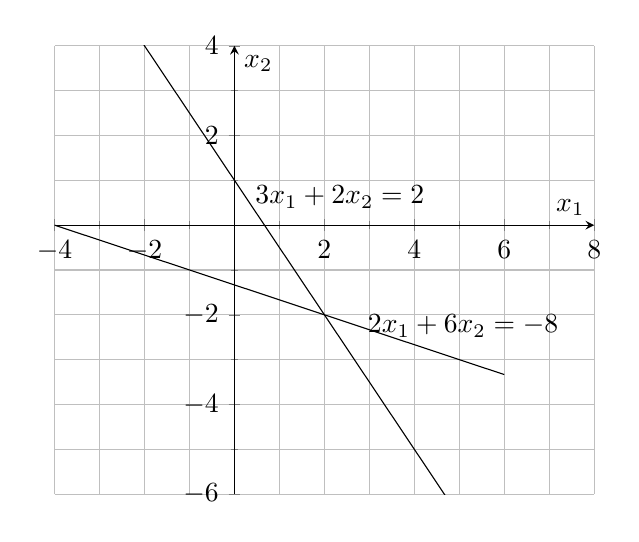
\begin{tikzpicture}
\begin{axis}[grid=both,ymin=-6,ymax=4,xmax=8,xmin=-4,
               minor tick num=1,axis lines = middle,xlabel=$x_1$,ylabel=$x_2$]
\addplot [domain=-4:6, samples=101]{-1.5*x+1} node[pos=0.425] (endofplotsquare) {};
\node [right] at (endofplotsquare) {$3x_1+2x_2=2$};
\addplot [domain=-4:6, samples=101]{-(1/3)*x-(8/6)} node[pos=0.675] (endofplotsquare2) {};
\node [right] at (endofplotsquare2) {$2x_1+6x_2=-8$};
\end{axis}
\end{tikzpicture}
\caption{Plots of the function $f_1$ and $f_2$ to visually obtain the intersection of the the two lines.}
\label{fig:example:interesction}
\end{figure}

%----------------------------------------------------------------------------------------
\section{Conjugate Gradient solver}
%----------------------------------------------------------------------------------------
For one examples of iterative solvers\index{iterative solvers}, we look into the most popular iterative method for solving large systems of linear equations. More details about iterative methods~\cite{olshanskii2014iterative,briggs2000multigrid}. The Conjugate Gradient (CG)\index{conjugate gradient} solver which was developed by Hestenes and Stiefel in 1952~\cite{hestenes1952methods}. The method solves linear equation systems with the form $\mathbf{A} \mathbf{x} = \mathbf{b}$. The matrix $\mathbf{A}$ has to be symmetric $\mathbf{A}^T = \mathbf{A}$ and positive-definite $\mathbf{x}^T \mathbf{A} \mathbf{x} > 0, \forall \mathbf{x}>0$. \\

We use the problem showed in Figure~\ref{fig:example:interesction} and define the system $\mathbf{A} \mathbf{x} = \mathbf{b}$ as
\begin{align*}
\mathbf{A} = \begin{pmatrix}
 3 & 2 \\ 2 & 6 
\end{pmatrix}, \mathbf{x}=\begin{pmatrix}
x_1 \\ x_2  
\end{pmatrix}, \text{ and }  \mathbf{b}=\begin{pmatrix}
2 \\ -8  
\end{pmatrix}\text{.}
\end{align*}
Since we know that solving that solving the matrix form can be expensive for large amounts of unknowns, the quadratic form, which is a function of the vector $\mathbf{x}$
\begin{align}
f(\mathbf{x}) = \frac{1}{2} \mathbf{x}^T A \mathbf{x} - b^T \mathbf{x} + c
\end{align}
can be minimized to find the solution for $\mathbf{x}$. Figure~\ref{fig:quadratic:plot} shows the plot of the quadratic form and Figure~\ref{fig:quadratic:contour} shows the contour plot of the quadratic form with the solution $(2,-2)$. To exemplify  the minimization to find the solution, we can place a golf ball at any position of the bowlish from of the quadratic form and the golf ball will roll to the solution, since the solution is the minimum of the quadratic form.\\

\begin{figure}[tb]
\begin{subfigure}{.75\textwidth}
\hfill
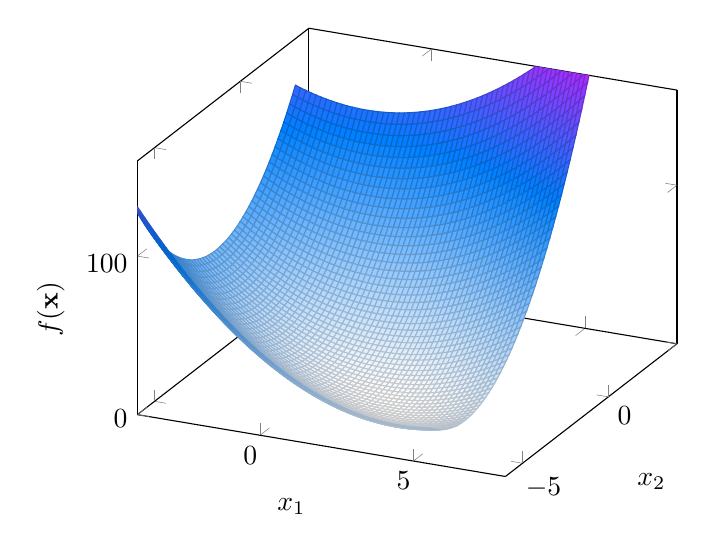
\begin{tikzpicture}
\begin{axis}[ymin=-6,ymax=4,xmax=8,xmin=-4,zmin=0,zmax=160,xlabel=$x_1$,ylabel=$x_2$,zlabel={$f(\mathbf{x})$}]
\addplot3[
    surf,
    colormap/cool,
    %shader=interp,
    %shader=flat,
    samples=60] 
    {x*(1.5*x+y)-2*x+y*(x+3*y)+8*y};
\end{axis}
\end{tikzpicture}
\hfill
\caption{Plot of the quadratic form $f(\mathbf{x})$ }
\label{fig:quadratic:plot}
\end{subfigure}
\\
\begin{subfigure}{.75\textwidth}
\hfill
\begin{tikzpicture}
\begin{axis}[ymin=-6,ymax=4,xmax=6,xmin=-4,xlabel=$x_1$,ylabel=$x_2$]
\addplot gnuplot[raw gnuplot,thick,mark=none]
    {
        unset surface;
        set cntrparam levels auto 10;
        set contour;
        set yrange [-6:4];
        splot [x=-4:6] x*(1.5*x+y)-2*x+y*(x+3*y)+8*y;
    };
\addplot[mark=*] coordinates {(2,-2)};
\end{axis}
\end{tikzpicture}
\hfill
\caption{Contour plot of the quadratic form $f(\mathbf{x})$}
\label{fig:quadratic:contour}
\end{subfigure}
\caption{Plot of the quadratic form $f(\mathbf{x})$ (\subref{fig:quadratic:plot}) and contour plot of the quadratic form $f(\mathbf{x})$ (\subref{fig:quadratic:contour}).}
\end{figure}

Now we want to mimic the metaphor of the rolling golf ball in a numerical sense. Therefore, we chose an arbitrary point $\mathbf{x}_0$ on the quadratic form and intend to slide down to the bottom of the bowl shape of the quadratic form to find the solution. Thus, we need to find the direction which decreases most. To find these, we use the gradient of the quadratic form
\begin{align}
f'(\mathbf{x})=\begin{pmatrix}
\frac{\partial }{\partial x_1} f(\mathbf{x}) \\
\frac{\partial }{\partial x_2} f(\mathbf{x}) \\
\vdots \\
\frac{\partial }{\partial x_n} f(\mathbf{x})
\end{pmatrix}\text{.}
\end{align}
Using the quadratic form, the gradient and applying some mathematics, one can show that the gradient reads as
\begin{align}
f'(\mathbf{x}) = \frac{1}{2} \mathbf{A}^T \mathbf{x} + \frac{1}{2} \mathbf{A} \mathbf{x}-\mathbf{b}
\end{align}
and for a symmetric matrix $\mathbf{A}$ the gradient reads as
\begin{align}
f'(\mathbf{x})= \mathbf{A}\mathbf{x}-\mathbf{b}\text{.}
\end{align}
Note that this course focus on the computer science and implementation aspects of the CG solver and for more details about the mathematics, we refer to~\cite{shewchuk1994introduction} where the very nice example for the introduction of the conjugate gradient method was adapted from. Figure~\ref{fig:gradient:field} plots the gradient field and one can see that the gradient at the solution $\mathbf{x}$ is zero. Thus, we can minimize the initial guess $\mathbf{x}_0$ such that the gradient $f'(x)=0$.\\

\begin{exercise}
To gain better understanding, we encourage you to follow the calculations in~\cite{shewchuk1994introduction} or even better try to do the altercations on your own and check them later in the reference.
\end{exercise}

\begin{figure}[tb]
\centering
\begin{tikzpicture}[scale=0.5]
\foreach \x in {-4,...,6} {
\foreach \y in {-6,...,4} {

\pgfmathsetmacro\mx{0.01*(3*\x+2*\y-2)};
\pgfmathsetmacro\my{0.01*(2*\x+6*\y+8)};

%\def\l{{sqrt(\u+\v)}};
%\node at (\x,\y) {\ml};
\draw[->,azure] (\x,\y) -- (\x+\mx,\y+\my);
}
}

\node[black] at (2,-2)  {\textcolor{black}{$\mathbf{x}$}};

\draw[->,thin,gray] (0,-7) -- (0,5);
\node[above] at (0,5) {\small $x_1$};
\draw[->,thin,gray] (-5,0) -- (7,0);
\node[above] at (7,0) {\small $x_2$};
\end{tikzpicture}
\caption{Plot of the gradient field  $f'(x)$ with the solution $\mathbf{x}$. }
\label{fig:gradient:field}
\end{figure}

To implement the metaphor of the rolling golf ball, we use the method of the steepest decent\index{steepest decent method}. In this method, we chose an random initial guess $\mathbf{x}_0$ and slide down to the bottom of the quadratic form $f(\mathbf{x})$ by taking a series of steps $\mathbf{x}_1,\mathbf{x}_2,\ldots$. For each step we go to the direction which $f$ decreases most which is the opposite of $f'(\mathbf{x}_i)$ which is $-f'(\mathbf{x}_i)= \mathbf{b}-\mathbf{A}\mathbf{x}_i$.

%----------------------------------------------------------------------------------------
\subsubsection{Method of the steepest decent}
%----------------------------------------------------------------------------------------
Before, we look into the method, we have to define two terms, see Figure~\ref{fig:skecth:error:residual}. Assume we know the solution $\mathbf{x}$ and we have our initial guess $\mathbf{x}_0$ we can define the error $\mathbf{e} = \mathbf{x}_0 - \mathbf{x}$ or more general for the $i$-th iteration as  $\mathbf{e}_i = \mathbf{x}_i - \mathbf{x}$. The residual $\mathbf{r}_i = \mathbf{b}-\mathbf{A}\mathbf{x}_i=-f'(\mathbf{x_i})$ which defines how far we are form the correct value for the right-hand side $\mathbf{b}$. Remember the metaphor of the golf ball sliding down to the bottom of the bowlish shape. This means for us now that we have to go along the line $\mathbf{r}_0$ to get closer to the bottom. Since we do not have gravity guiding us to the bottom. we have to decide on how long we want to go along the line $\mathbf{r}_0$.\\

\begin{figure}[tb]
\centering
\begin{tikzpicture}
\begin{axis}[ymin=-6,ymax=4,xmax=6,xmin=-4,xlabel=$x_1$,ylabel=$x_2$]
\addplot gnuplot[raw gnuplot,thick,mark=none]
    {
        unset surface;
        set cntrparam levels auto 10;
        set contour;
        set yrange [-6:4];
        splot [x=-4:6] x*(1.5*x+y)-2*x+y*(x+3*y)+8*y;
    };
\addplot[mark=*] coordinates {(2,-2)};
\node[below] at (2,-2) {$\mathbf{x}$};
\addplot[mark=*] coordinates {(-2,-2)};
\node[below,black] at (-2,-2) {$\mathbf{x}_0$};
\draw (2,-2) -- (-2,-2);
\node[below] at (-0,-2) {$\mathbf{e}_0$};
\draw (-2,-2) -- (8,12);
\node[left] at (-0,1) {$\mathbf{r}_0$};
\end{axis}
\end{tikzpicture}
\caption{Visualization of the error $\mathbf{e}$ and the residual $\mathbf{r}$. We have to determine how long we should go along the residual line within one iteration. }
\label{fig:skecth:error:residual}
\end{figure}

So we have to find $\alpha$ for how long we go in the direction of the steepest decent $\mathbf{x}_1 = \mathbf{x}_0 + \alpha \mathbf{r}_0$. Figure~\ref{fig:plane:plot} visualized the plane defined by $\mathbf{x}_1 = \mathbf{x}_0 + \alpha \mathbf{r}_0$ and the quadratic form $f(\mathbf{x})$. Next, we look at the intersection of the two surfaces which is some parabola, see Figure~\ref{fig:plane:intersection}. Now, we have to find the minimum of the parabola $\frac{d}{d\alpha} f(\mathbf{x}_0 + \alpha \mathbf{r}_0) = 0$ to determine the optimal value for $\alpha$. Applying the chain rule results in $\frac{d}{d\alpha} f(\mathbf{x}_0 + \alpha \mathbf{r}_0)= f'(\mathbf{x}_0 + \alpha \mathbf{r}_0)^T \mathbf{r}_0$. This expression is zero if and only if the two vectors are orthogonal. We can do some calculations
\begin{align}
\mathbf{r}^T_1 \mathbf{r}_0 &= 0 \\
(\mathbb{b}-\mathbf{A} \mathbf{x}_1)^T \mathbf{r}_0 & = 0 \\
(\mathbb{b}-\mathbf{A} (\mathbf{x}_0 + \alpha \mathbf{r}_0))^T \mathbf{r}_0 & = 0 \\
(\mathbf{b}- \mathbf{A} \mathbf{x}_0)^T \mathbf{r}_0 - \alpha(\mathbf{A}\mathbf{r}_0)^T \mathbf{r}_0 &= 0 \\
(\mathbf{b}- \mathbf{A} \mathbf{x}_0)^T \mathbf{r}_0  &= \alpha(\mathbf{A}\mathbf{r}_0)^T \mathbf{r}_0 \\
\mathbf{r}^T_0 \mathbf{r}_0 &= \alpha \mathbf{r}^T_0 (\mathbf{A}\mathbf{r}_0) \\
\alpha &= \frac{\mathbf{r}^T_0 \mathbf{r}_0}{\mathbf{r}^T_0 \mathbf{A}\mathbf{r}_0}
\end{align}
to compute $\alpha$. Note that this course focus on the computer science and implementation aspects of the CG solver and for more details about the mathematics, we refer to~\cite{shewchuk1994introduction} where the very nice example for the introduction of the conjugate gradient method was adapted from. Figure~\ref{fig:previous:step} shows the first iteration and how long to go along the the residual line to the next guess of the solution $\mathbf{x}_1$ and we clearly see that the gradient is to $\mathbf{x}_0$.\\

\begin{exercise}
To gain better understanding, we encourage you to follow the calculations in~\cite{shewchuk1994introduction} or even better try to do the altercations on your own and check them later in the reference.
\end{exercise}

\begin{figure}
\centering
\begin{tikzpicture}
\begin{axis}[ymin=-6,ymax=4,xmax=6,xmin=-4,xlabel=$x_1$,ylabel=$x_2$]
\addplot gnuplot[raw gnuplot,thick,mark=none]
    {
        unset surface;
        set cntrparam levels auto 10;
        set contour;
        set yrange [-6:4];
        splot [x=-4:6] x*(1.5*x+y)-2*x+y*(x+3*y)+8*y;
    };
\addplot[mark=*] coordinates {(2,-2)};
\node[below] at (2,-2) {$\mathbf{x}$};
\addplot[mark=*] coordinates {(-2,-2)};
\node[below] at (-2,-2) {$\mathbf{x}_0$};
\addplot[mark=*] coordinates {(0.08,-0.61333)};
\draw (-2,-2) -- (0.08,-0.61333);
\node[below] at (0.08,-0.61333) {$\mathbf{x}_1$};
\draw[->] (0.08,-0.61333) -- (0.1*-2.98666667, 0.1*4.48); 
%\node[left] at (-0,1) {$\mathbf{r}_0$};
\end{axis}
\end{tikzpicture}
\caption{first iteration and how long to go along the the residual line to the next guess of the solution $\mathbf{x}_1$ and we clearly see that the gradient is to $\mathbf{x}_0$.}
\label{fig:previous:step}
\end{figure}

\begin{figure}[tb]
\begin{subfigure}{.75\textwidth}
\hfill
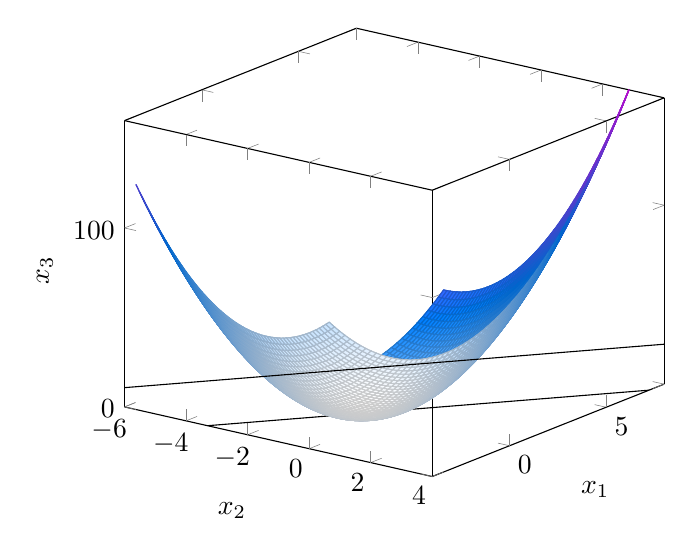
\begin{tikzpicture}
\begin{axis}[ymin=-6,ymax=4,xmax=8,xmin=-4,zmin=0,zmax=160,xlabel=$x_1$,ylabel=$x_2$,zlabel=$x_3$,view={53}{338}]
\addplot3[
    surf,
    colormap/cool,
    %shader=interp,
    %shader=flat,
    samples=60] 
    {x*(1.5*x+y)-2*x+y*(x+3*y)+8*y};
    \addplot3[
    domain=-4:10,
    samples = 60,
    samples y=0,
]
({-2+12*x},
{-2+8*x},
{x});
\addplot3[
    surf,
    colormap/cool,
    %shader=interp,
    %shader=flat,
    samples=60] 
    {x*(1.5*x+y)-2*x+y*(x+3*y)+8*y};
    \addplot3[
    domain=-4:10,
    samples = 60,
    samples y=0,
]
({-2+12*x},
{-2+8*x},
{25+x});
\end{axis}
\end{tikzpicture}
\hfill
\caption{Plot of the quadratic form $f(\mathbf{x})$ and the area of the line search $\mathbf{x}_1 = \mathbf{x}_0 + \alpha \mathbf{r}_0$ }
\label{fig:plane:plot}
\end{subfigure}
\\
\begin{subfigure}{.75\textwidth}
\hfill
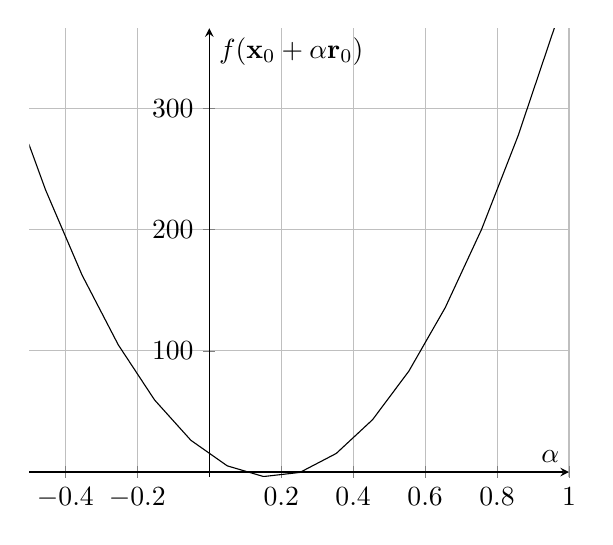
\begin{tikzpicture}
\begin{axis}[xmin=-0.5,xmax=1,xlabel=$\alpha$,ylabel=$f(\mathbf{x}_0 + \alpha \mathbf{r}_0)$,axis lines = middle, grid= both]
\addplot[samples=100]{(-2+12*x)*(1.5*(-2+12*x)+(-2+8*x))-2*(-2+12*x)+(-2+8*x)*((-2+12*x)+3*(-2+8*x))+8*(-2+8*x)};
\end{axis}
\end{tikzpicture}
\hfill
\caption{Contour plot of the quadratic form $f(\mathbf{x})$}
\label{fig:plane:intersection}
\end{subfigure}
\caption{Plot of the two surfaces (\subref{fig:plane:plot}) and resulting parabola of the intersection of these two surfaces (\subref{fig:plane:intersection}).}
\end{figure}

Now, we extend this example to the algorithm to iterate to the solution of the linear equation system. Figure~\ref{fig:algorithm:cg} shows the flow chart of the conjugate gradient solver. First, we have to check if the residual is close to the tolerance $\epsilon$, if so, we guessed $\mathbf{x}_0$ close enough to the solution. If not, the residual $\mathbf{r}_i$ is evaluated. Next, we compute $\alpha_i$ and the new guess $\mathbf{x}_{i+1}$. Now, we check if the residual with respect to $\mathbf{x}_{i+1}$ is close enough to the tolerance, if so, we return the solution. If not, we proceed with the next iteration. Algorithm~\ref{alg:cg} shows the pseudo code for the CG method. Here more implementation details as in the flow chart are provided. Figure~\ref{fig:line:search} shows the first five iterations of the CG algorithm with the initial guess $\mathbf{x_0}=(-2,-2)^T$ and the solution $\mathbf{x}_5=(1.93832964, -2.)^T$. Fore more details on iterative solver, we refer to~\cite{barrett1994templates}.

\begin{figure}[tb]
    \centering
	\begin{tikzpicture}[node distance=1.125cm, scale=0.75, transform shape]
	\node (start) [startstop] {Start}; 
	\node (n0) [process, below of=start] { $\mathbf{r}_0 = \mathbf{b} - \mathbf{A} \mathbf{x}_0$};
	\node (dec1) [decision, below of=n0 , yshift=-1.cm] { $\vert\mathbf{r}_0\vert < \epsilon$ };
	\node (n1) [process, right of=dec1, xshift=3.cm] { return $\mathbf{x}_0$};
	\node (stop) [startstop, right of=n1, xshift=4.cm] {Finished}; 
	\node (n2) [process, below of=dec1, yshift=-1.cm] { $\mathbf{r}_i = \mathbf{b} - \mathbf{A} \mathbf{x}_i$ };
	\node (n3) [process, below of=n2, yshift=-1.cm] { $\alpha_i = \frac{\mathbf{r}^T_0 \mathbf{r}_0}{\mathbf{r}^T_0 \mathbf{A}\mathbf{r}_0}$ };
	\node (n4) [process, below of=n3, yshift=-1.cm] { $\mathbf{x}_{i+1} = \mathbf{x}_i \alpha_i \mathbf{r}_i$ };
	\node (dec2) [decision, below of=n4 , yshift=-1.cm] {  $\mathbf{r}_i < \epsilon$ };
	\node (n5) [process, right of=dec2, xshift=3.cm] { return $\mathbf{x}_i$};
	\node (n6) [process, left of=dec2, xshift=-3.cm] { $i++$};
	%lines
	\draw [->] (start) -- (n0);
	\draw [->] (n0) -- (dec1);
	\draw [->] (n1) -- (stop);
	\draw [->] (dec1) -- node[anchor=north] {yes} (n1); 
	\draw [->] (dec1) -- node[anchor=west] {no}  (n2);
	\draw [->] (n2) -- (n3);
	\draw [->] (n3) -- (n4);
	\draw [->] (n4) -- (dec2);
	\draw [->] (dec2) -- node[anchor=north] {yes} (n5); 
	\draw [->] (n5) -- ++(5.25,0) -- (stop);
	\draw [->] (dec2) -- node[anchor=north] {no}  (n6);
	\draw [->] (n6) -- ++(0,6.5) -- (n2);
	\end{tikzpicture}
	\caption{Flow chart for the Conjugate Gradient method to solve $\mathbf{M}\mathbf{x}=\mathbf{b}$.}
	\label{fig:algorithm:cg}
\end{figure}

\begin{algorithm}
\begin{algorithmic}
\State $\mathbf{r_0} = \mathbf{b} - \mathbf{A} \mathbf{x}_0$
\If {$\mathbf{r}_0< \epsilon$}
    \Return $\mathbf{x}_0$
\EndIf
\State $\mathbf{p}_0=\mathbf{r}_0$
\State $k=0$
\While{true} 
\State $\alpha_k = \frac{\mathbf{r}_k^T\mathbf{r}_k}{\mathbf{p}_k^T\mathbf{A}\mathbf{p}_k}$
\State $ \mathbf{x}_{k+1} = \mathbf{x}_k + \alpha_k \mathbf{p}_k$
\State $ \mathbf{r}_{k+1} = \mathbf{r}_k - \alpha_k \mathbf{p}_k$
\If { $\mathbf{r}_{k+1}< \epsilon$}
   \State exit loop
\EndIf
\State $\beta_k = \frac{\mathbf{r}_{k+1}^T\mathbf{r}_{k+1}}{\mathbf{r}_k^T\mathbf{r}_k}$
\State $\mathbf{p}_{k+1}=\mathbf{r}_{k+1} + \beta_k \mathbf{p}_k$
\State $k=k+1$
\EndWhile
\State return $\mathbf{x}_{k+1}$
\end{algorithmic}
\caption{Implementation of the Conjugate Gradient method with some additions where the factor $\beta$ is computed.}
\label{alg:cg}
\end{algorithm}

%\item $\mathbf{r_0} = \mathbf{b} - \mathbf{A} \mathbf{x}_0$
%\item If $\mathbf{r}_0< \epsilon$ return  $\mathbf{x}_0$
%\item $\mathbf{p}_0=\mathbf{r}_0$
%\item $k=0$
%\item $\alpha_k = \frac{\mathbf{r}_k^T\mathbf{r}_k}{\mathbf{p}_k^T\mathbf{A}\mathbf{p}_k}$
%\item $ \mathbf{x}_{k+1} = \mathbf{x}_k + \alpha_k \mathbf{p}_k$
%\item $ \mathbf{r}_{k+1} = \mathbf{r}_k - \alpha_k \mathbf{p}_k$
%\item If $\mathbf{r}_{k+1}< \epsilon$ exit loop
%\item $\beta_k = \frac{\mathbf{r}_{k+1}^T\mathbf{r}_{k+1}}{\mathbf{r}_k^T\mathbf{r}_k}$
%\item $\mathbf{p}_{k+1}=\mathbf{r}_{k+1} + \beta_k \mathbf{p}_k$
%\item $k=k+1$
%\item go to (e)
%return $\mathbf{x}_{k+1}$

\begin{figure}
\centering
\begin{tikzpicture}
\begin{axis}[ymin=-6,ymax=4,xmax=6,xmin=-4,xlabel=$x_1$,ylabel=$x_2$]
\addplot gnuplot[raw gnuplot,thick,mark=none]
    {
        unset surface;
        set cntrparam levels auto 10;
        set contour;
        set yrange [-6:4];
        splot [x=-4:6] x*(1.5*x+y)-2*x+y*(x+3*y)+8*y;
    };
\addplot[mark=*] coordinates {(2,-2)};
\node[above] at (2,-2) {$\mathbf{x}$};
\addplot[mark=*] coordinates {(-2,-2)};
\node[below] at (-2,-2) {$\mathbf{x}_0$};
\addplot[mark=*] coordinates {(0.08,-0.61333)};
\draw (-2,-2) -- (0.08,-0.61333);
\node[below] at (0.08,-0.61333) {$\mathbf{x}_1$};
\addplot[mark=*] coordinates {(1.00444444, -2.)};
\draw (0.08,-0.61333) -- (1.00444444, -2.);
\node[below] at (1.00444444, -2.) {$\mathbf{x}_2$};
\addplot[mark=*] coordinates {(1.52213333, -1.65487407)};
\draw (1.00444444, -2.) -- (1.52213333, -1.65487407);
\node[above] at (1.52213333, -1.65487407) {$\mathbf{x}_3$};
\addplot[mark=*] coordinates {(1.75221728, -2.)};
\draw (1.52213333, -1.65487407) -- (1.75221728, -2.);
\node[below] at (1.75221728, -2.) {$\mathbf{x}_4$};
\draw (1.75221728, -2.) -- (1.8810643 , -1.91410199);
\draw (1.8810643 , -1.91410199) -- (1.93832964, -2.);
\end{axis}
\end{tikzpicture}
\caption{Visualization of the line search for the first five iterations of the Conjugate Gradient algorithm with the solution $\mathbf{x}_5=(1.93832964, -2.)^T$.}
\label{fig:line:search}
\end{figure}

\newpage
\begin{exercise}
Implement the conjugate gradient algorithm using Blaze library. This code produces a matrix $\mathbf{A}$ and a vector $\mathbf{b}$, such that the vector $\mathbf{x}$ is the solution for  $\mathbf{A} \mathbf{x} = \mathbf{b}$
\begin{lstlisting}[language=C++]
 for(int i=0; i<N; ++i) {
        A(i,i) = 2.0;
        b[i] = 1.0*(1+i);
        x[i] += x[i-1];
    }
\end{lstlisting}
You can use the matrix $\mathbf{A}$ and the vector $\mathbf{b}$ as the input of your CG implementation and compare your solution with the vector $\mathbf{x}$ to validate your code. You should not use this vector as the input of the CG algorithm, since your code might stop at step (2) already.
\end{exercise}

\newpage
\theendnotes